%%%%%%%%%%%%%%%%%% USAGE INSTRUCTIONS %%%%%%%%%%%%%%%%%%
% - Compile using LuaLaTeX and biber, unless there is a particular reason not to. Do not use the older LaTex/PDFLaTeX or BibTeX. (The fonts won't work correctly.)
% - Font and the report 'year' must be specified when all \documentclass or the template won't work correctly. (There's no error checking/default cases!)
% - For best performance save images/graphics as PDF files, not as png/jpg/eps. This makes no difference to how images are inserted using \includegraphics.
% - As many further packages as wanted can be loaded. Below are just an example set. Note that template itself loads a number of packages, including hyperref.
% - References are handed using biblatex.
% - Link to the presentation of theses policy: https://documents.manchester.ac.uk/DocuInfo.aspx?DocID=2863

%%%%%%%%%%%%%%%%%% META DATA SETUP %%%%%%%%%%%%%%%%%%
% This is where the document title and author are set. Other details for the title page are set later
% Note that if/when you edit these you may need to 'Recompile from scratch' to get the changes to display in the PDF. (In Overleaf, select the down arrow to the right of the 'Recompile' button)
\begin{filecontents*}{\jobname.xmpdata}
    \Title{Development of Two Wheel Self Balancing Line Following Robot} % title of your thesis
    \Author{Winston Scott 107067151} % should be student number rather than name to help with annoymous marking
    \Language{en-GB}
    \Copyrighted{True}
    % More meta-data fielda can be added here if wanted, see https://ctan.org/pkg/pdfx?lang=en for fields
    \end{filecontents*}
    %%%%%%%%%%%%%%%%%% DOCUMENT SETUP %%%%%%%%%%%%%%%%%%
    \documentclass{uom_eee_dissertation_casson} 
    %%%%%%%%%%%%%%%%%% PACKAGES AND COMMANDS %%%%%%%%%%%%%%%%%%
    % Packages
    \usepackage{graphicx,psfrag,color} % for postscript graphics files
        \graphicspath{ {./images/} }   % where to look for images
    \usepackage{amsmath}               % assumes amsmath package installed
        \allowdisplaybreaks[1]         % allow eqnarrays to break across pages
    \usepackage{amssymb}               % assumes amsmath package installed 
    \usepackage{url}                   % format hyperlinks correctly
    \usepackage{rotating}              % allow portrait figures and tables
    \usepackage{multirow}              % allows merging of rows in tables
    \usepackage{lscape}                % allows pages to be typeset in landscape mode
    \usepackage{tabularx}              % allows fixed width tables
    \usepackage{verbatim}              % enhanced version of built-in verbatim environment
    \usepackage{footnote}              % allows more control over footnote environments
    \usepackage{float}                 % allows H option on floats to force here placement
    \usepackage{booktabs}              % improve table line spacing
    \usepackage{lipsum}                % for adding dummy text here
    \usepackage[base]{babel}           % for proper hypthenation in lipsum sections
    \usepackage{subcaption}            % for multiple sub-figures in a single float
    % Add your packages here
    %\usepackage{pdfcomment}            % for alt text for accessibility
    \usepackage{booktabs}              % for better looking tables
    % Then to add images use:
    % \pdftooltip{\includegraphics[width=0.5\textwidth]{image.pdf}}{Alt-text here}
    % This makes the text in the image non-select-able though (assuming it's a vector file)
    
    % Custom commands
    \newcommand{\degree}{\ensuremath{^\circ}}
    \newcommand{\sus}[1]{$^{\mbox{\scriptsize #1}}$} % superscript in text (e.g. 1st)
    \newcommand{\sub}[1]{$_{\mbox{\scriptsize #1}}$} % subscript in text
    \newcommand{\sect}[1]{Section~\ref{#1}}
    \newcommand{\fig}[1]{Fig.~\ref{#1}}
    \newcommand{\tab}[1]{Table~\ref{#1}}
    \newcommand{\equ}[1]{(\ref{#1})}
    \newcommand{\appx}[1]{Appendix~\ref{#1}}
    %%%%%%%%%%%%%%%%%% REFERENCES SETUP %%%%%%%%%%%%%%%%%%
    % Setup your references here. Change the reference style here if wanted
    \usepackage[style=ieee,backend=biber,backref=true,hyperref=auto]{biblatex}
    % Note backref=true adds a page number (and hyperlink) to each reference so you can easily go back from the references to the main document. You may prefer backref=false if you need to stick strictly to a given reference style
    % Fixes which can't be applied in the .cls file
    \DefineBibliographyStrings{english}{backrefpage = {cited on p\adddot},  backrefpages = {cited on pp\adddot}}
    %  \renewcommand*{\bibfont}{\large}
    % Add more .bib files here if wanted
    \addbibresource{References.bib}
    
    %%%%%%%%%%%%%%%%%% START DOCUMENT %%%%%%%%%%%%%%%%%%
    % Don't edit these lines, title and author are automatically taken from the document meta-data defined above
    \begin{document}
    \makeatletter
    \title{\xmp@Title}
    \studentid{\xmp@Author}
    \makeatother
    
    % Set the below yourself
    \course{Mechatronics and Robotics Engineering}  % "Master of Science in" is added automatically
                                                    % Our courses are: Advanced Control and Systems Engineering, Advanced Control and Systems Engineering with Extended Research, Communications and Signal Processing, Communications and Signal Processing with Extended Research, Electrical Power Systems Engineering, Advanced Electrical Power Systems Engineering, Renewable Energy and Clean Technology, Renewable Energy and Clean Technology with Extended Research
    \submitdate{2025}                               % regulations ask only for the year, not month
    \wordcount{1000}		                    % use \wordcount{} to set the count, \thewordcount to print in the text
    \maketitle

    %%%%%%%%%%%%%%%%%% LISTS OF CONTENT %%%%%%%%%%%%%%%%%%
    \uomtoc
    % other lists are not required, but can include \uomlof and \uomlot if really want to

    %%%%%%%%%%%%%%%%%% ABSTRACT %%%%%%%%%%%%%%%%%%
    \begin{abstract} % put abstract here. Limit is 1 page.
    The highly dynamic Two Wheel Self Balancing Robot 
    (TWSB) has a large exploration space for developing high level 
    control strategies. 
    This report presents the design decisions and algorithms developed for
    an autonomous line racing TWSB robot utilizing a monocular vision system with low cost hardware. 
    System identifications techniques are used to explore
    cascaded PID and LQG control strategies.
    A trajectory generation algorithm is proposed based on drivability, confidence 
    and prominence of the detected line from a camera used as an intensity sensor. 
    The performance of the the system is shown to be robust to different race tracks which
    surface texture variation, lighting conditions, high speed straights and tight curves. 

    \begin{figure}[H]
    \centering
    \includegraphics[width=\textwidth]{CurveSequence.pdf}
    \caption{Tracking a tight chicane at high speed}
    \end{figure}

  \end{abstract}%
  \clearpage
  %%%%%%%%%%%%%%%%%% SECTION 1 %%%%%%%%%%%%%%%%%%
    \section{Introduction}
    The TWSB system is an example of a non-linear, under-actuated system that is inherently unstable.
    Compared to a differential drive mobile platform, the TWSB's dynamics are more complex as
    it is fundamentally a 3D system. Control of this extra degree of freedom enables a wider range 
    of autonomous behaviors to be explored. Significant research, both in simulation[][] and application[][][] 
    has been done on the similarly unstable 1DOF inverted pendulum on a cart as a bench mark for control techniques \cite{boubaker2013inverted}. 
    Its low degree of freedom however is a limitation for real world applications like the service industry, 
    which is dominated by wheeled robots. Whilst recently bipeds[][][] have gained attention 
    due to the purposed ability to ingrate in human centric environments, 
    their autonomous navigation is still an area of active research[]. 
    
    The TWSB robot finds a middle ground between the simplify of planar wheeled robots and the
    behavioral complexity of bipeds.Its low cost and high mobility make is a suitable platform 
    for research in the field of mobile robotics.
    
    Amongst the early works on the TWSB system,\cite{grasser2002joe} achieved teleoperation on flat ground. 
    This was implemented using a FPGA based DSP system, which by decoupling the balancing and steering torques 
    state-space control  is able to effectively navigating and turn on the spot. 
    \cite{kim2005dynamic} formulates a higher fidelity dynamical model of the wheel inverted pendulum, 
    using Kane's method in 3DOF space, and considers the limitations on performance of the robot on an 
    inclined plane based on its physical design.[]'s model accounts for the coriolis effect arising by nature of rotation about the Z axis, or yaw rate. 
    Advances in price-to-performance of emmbeded systems and breakthroughs in MEMS sensors \cite{MEMS} have since allowed 
    \cite{diaz2023ros} \cite{juang2013design} \cite{} to similarly obtain remote control of the TWSB system using a low powered microcontroller.
    With a stable mobile platform and available computational resources, many works
    
    This paper presents the design of a TWSB robotic platform, capable of autonomously navigating indoor line track. 
    The line is taken to be of a significant contrast to the environment and computer vision algorithms are used to 
    locate it. A racing algorithm is proposed based on 3 key metrics of the line; drivability, confidence and prominence.

    [] Utilizes a camera as a matrix of binary intensity sensors and a rule based algorithm to successful track 
    a line whilst balancing. [] Trained an end to end neural network to perform the same task and [] proposes 
    a convolution neural network based approach which utilizes all of the cameras RDB-D data to be able to 
    autonomously navigate with human-centric social behavior. 
    To the same end, [][][] develop wheeled robot navigation and realtime lane segmentation using 
    geometric computer vision techniques. 
    [][] build a online data driven model of the mobile system and emmbeded it in a Model Predictive Controller (MPC). 
    This adaptive control strategy is shown to be robust to un-modeled environment and plant dynamics, 
    allowing for autonomous aggressive maneuvers. 
    Whilst major success has been achieved by linearization of the dynamics of classic inverted pendulum, 
    [][] show that by using non-linear control strategies such as backstepping or sliding mode control
    the system can be made to stabilize on an inclined plane and even limbo under a bar.


    \pagebreak{}

  %%%%%%%%%%%%%%%%%% SECTION 2 %%%%%%%%%%%%%%%%%%
    \section{Mathematical Modeling} % edit section heading as appropriate
    \subsection{DC Motor Model}    
    \begin{figure}[H]
        \centering
            \includegraphics[width=0.75\textwidth]{Diagrams/DcMotorModel.pdf}
        \caption{Gearbox DC Motor Model Diagram}
    \end{figure}
    The system is driven by two independently voltage controlled DC motors through 
    planetary gearboxes, as is shown in Fig(2). 
    DC motors execute a torque $t_r$, proportional to the armature current $i_a$,
    when a voltage $V_a$ is applied.
    The ratio of motors inductance $L_a$ and resistance $R_a$ determine the
    time constant $\tau_e$ of the motor. That is the time it takes 
    for $i_a$ to reach 63.2\% of its final value. []
    The gear ratio $n=N_2/N_1$ which amplifies the viscous damping coefficient 
    $B_G$ and the moment of inertia $J_G$ with respect to the motor is obtained by
    $J_{\text{eq}} = J_G + J_r \cdot n^2$ and $B_{\text{eq}} = B_G \cdot n$.

    The speed of the gearbox, $\dot\phi_w$ is related to the armature voltage 
    by the well-known[] transfer function
    \begin{equation}
        \begin{aligned}
            \frac{\Omega_w \left(s\right)}{V_a \left(s\right)}=\frac{K_t }{s^2 \cdot L_a R_a +\;s\left(R_a \cdot J_{\mathrm{eq}} +B_{\mathrm{eq}} \cdot L_a \right)+K_t {\cdot K}_e +R_a \cdot B_q }\cdot\frac{1}{n}
        \end{aligned}
    \end{equation}
    Where $\Omega_w$ is the laplace transform of the output speed, $J_r$ is 
    the moment of inertia of the the rotor.
    The rotors viscous damping $B_r$ is assumed to be negligible, as is $B_G$. 
    For small motors, $t\tau_e$ is small hence $L_a << R_a$, [][], and the motor can be 
    approximated as a first order system as
    \begin{equation}
        \begin{aligned}
            \frac{\Omega_w \left(s\right)}{V_a \left(s\right)}=\frac{K_t }{s\cdot R_a + \left(J_G +{J_r \cdot n}^2 \right)+K_t K_e }\cdot\frac{1}{n}
        \end{aligned}
    \end{equation}

    \pagebreak{}

    \subsection{2DOF System Model}

    \begin{figure}[H]
        \includegraphics[width=\textwidth]{Diagrams/ModelingDiags.pdf}
        \caption{2DOF Model}
    \end{figure}

    The TWSB robot is modeled as two separate 2DOF systems as shown in fig(4), 
    namely a wheeled inverted pendulum (WIP) and a differential drive robot (DDMR).
    It however exits in a 3D space, and for the purposes of this paper must be able to rotate about the inertial Z axis. 
    [] Shows that that is possible to separate the steering control from the balance control 
    without linear velocity and direction angular velocity being constrained too much. 
   

    The system equations of motion in the WIP case are developed through the Lagrangian Method [][][] are shown to be 
    
    The system of equations () are linearized around the equilibrium point $\theta\approx 0$  and after standard algebraic manipulation the 
    2DOF state space representation of the system is given by eq(6).


   
    \pagebreak{}

    \section{System Design}
        \begin{figure}[H]
            \includegraphics[width=\textwidth]{DesingImgs/bBot Drawing v3.pdf}
            \caption{CAD Drawing of the TWSB system}
        \end{figure}

        The TWSB body is 3D printed out of PLA plastic in 3 parts for minimal assembly.
        The battery pack is quickly swappable and both it and the electronics sub assembly 
        are soft-mounted in a roll cage like housing for protection against impacts. 
        \begin{figure}[H]
            \centering
            \includegraphics[width=0.55\textwidth]{Diagrams/SystemOverview.pdf}
            \caption{System Overview}
        \end{figure}

        Two brushed DC motors are powered by an H-Bridge IC, DRV7783. 
        The STM32F411RE Microcontroller Unit (MCU) is used to control the 
        motors and monitor the 6 Axis Inertial Measurement Unit (IMU) over I2C. It communicates with the 
        Raspberry Pi 5 over UART via a custom ASCII protocol discussed in section 2.4. 
        The system is powered by a 12V nominal Li-ion Battery pack. A USB-C CC-CV charger is used for quick 
        and accessible recharging, critical for mobile robotics applications. 
        Battery voltage is monitored by the MCU and the pack is protected by a BMS and a 3A poly-fuse.
        A simple circuit adapted from[] is used to safely load share between the battery pack and the charger.

        \pagebreak{}
        \subsection{System Identification}
        A series of experiments are conducted in order to obtain an estimate transfer function of the motors
        
        \begin{table}[H]
            \centering
                \begin{tabular}{|r|c|c|c|c|c|c|}
                    \hline 
                    Gear Ratio & Rated Torque & Rated Speed  & Rated Current & Stall Current [A] & Stall Torque \\
                    \hline
                     1:20  & 0.39 [RPM] & 400 [mA] & 500 [Nm/kg] & 2  [A] & 0.15 [Nm/Kg] \\
                    \hline
                \end{tabular}
                \caption{Manufacturer Provided Motor Parameters}
        \end{table}
        A realtime data aquististion and analysis software system developed in python, is used as test bench setup 
        shown in fig(6), a series of reference ramp, step, sine and chirp inputs are applied to each of the DC motors.  
        \begin{figure}[H]
            \centering
            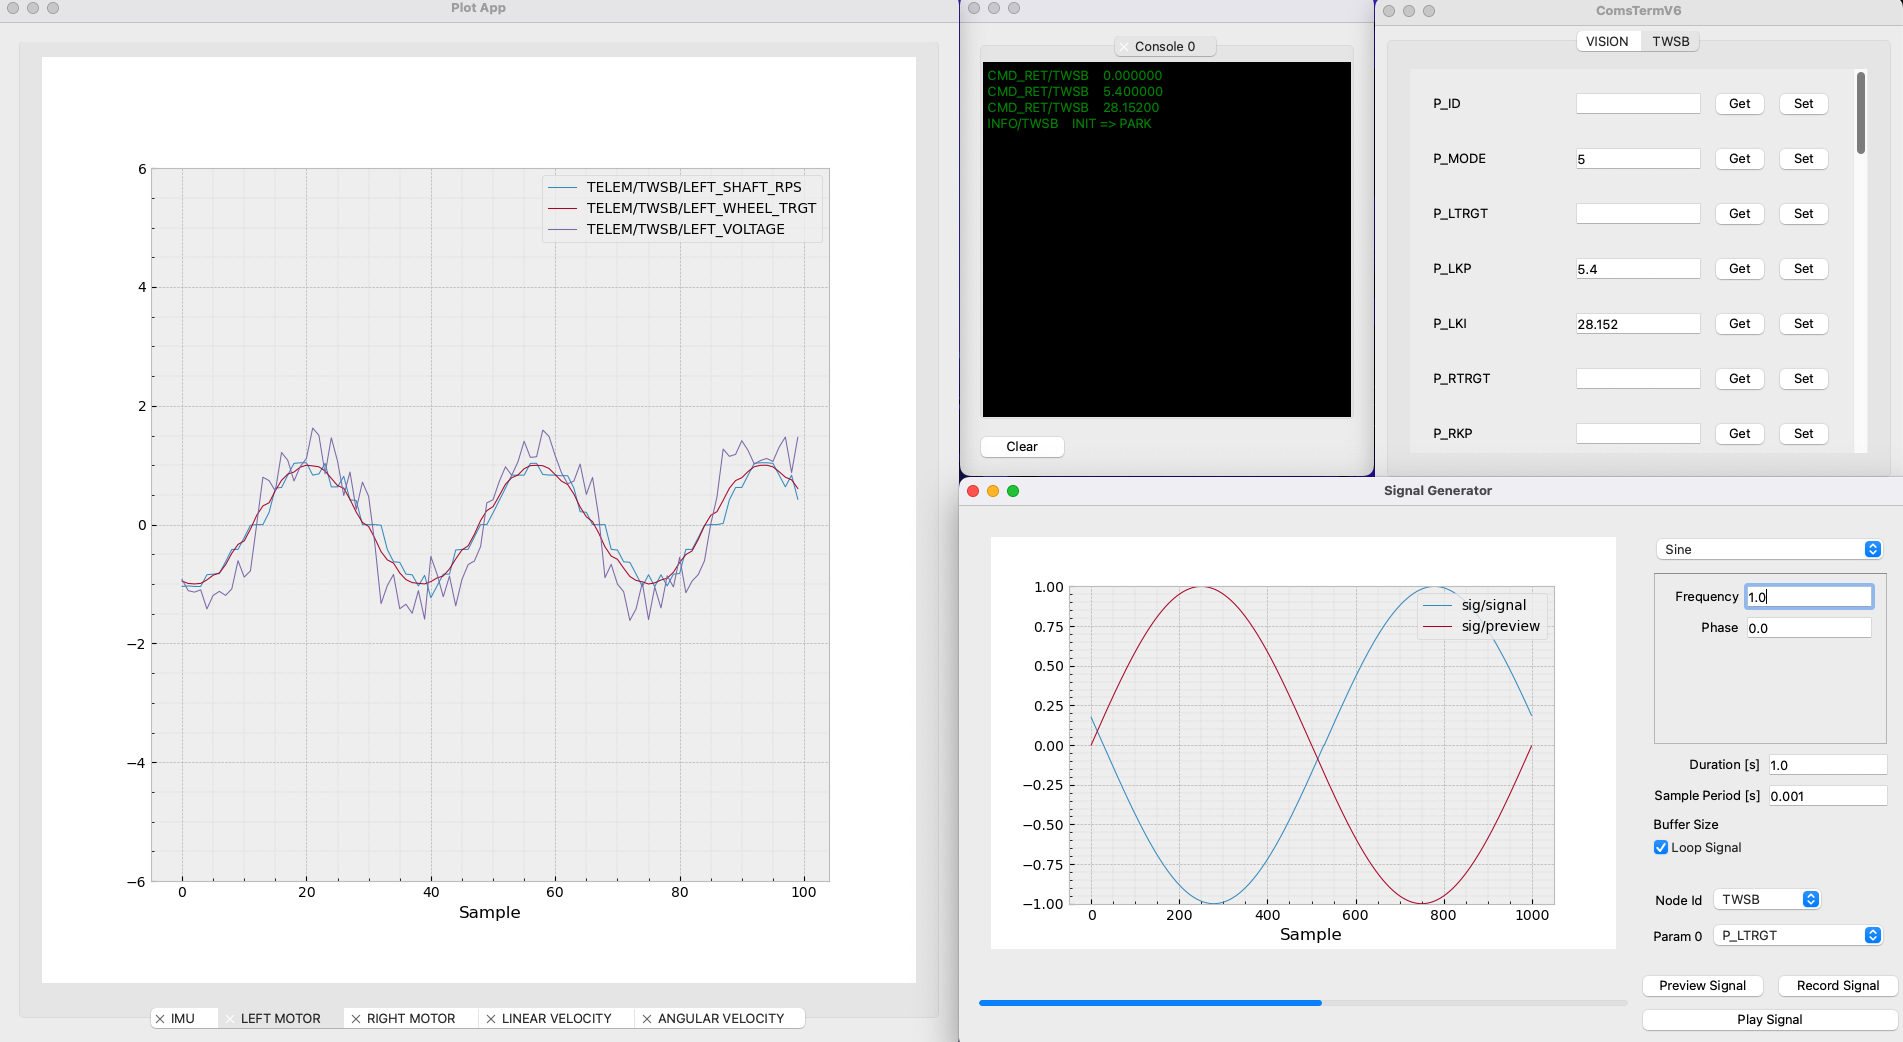
\includegraphics[height=0.45\textwidth]{SysIDMotorSetUp.png}
            \caption{System Identification Testbench Setup}
        \end{figure}
     
        \begin{figure}[H]
            \centering
            \subfloat{
                \includegraphics[width=0.3\textwidth]{Graphs/openstep.pdf}
            }
                \subfloat{
                \includegraphics[height=0.2\textwidth]{Graphs/speed_voltage_DCMotor.pdf}
            }
            \subfloat{
                \includegraphics[width=0.3\textwidth]{Graphs/openChirp.pdf}
            }
            \caption{Open Loop Speed Voltage experiments}
        \end{figure}    
        The transfer function of the motor is obtained by fitting the data to a first order system 
        with 95\% confidence intervals whose transfer function is given by eq(7).
        \begin{equation}
            \begin{aligned}
                \frac{\Omega_w \left(s\right)}{V_a \left(s\right)}=\frac{0.1}{s+0.9}
            \end{aligned}
        \end{equation}

        \pagebreak{}
        \subsubsection{Parameters }
        The system parameters are given in table(1). 
        The mass of the sub-components obtained by weighing,
        and estimates of the 3D printed parts mass are given by the slicer software. 
        The CAD Model computes the center of mass using these values and the COM is identified in fig(6).
        The using the approximate model as in fig(2) the moment of inertial is computed from standard formulas.
        \begin{table} [H]
            \centering
            \begin{tabular}{|c|c|c|c|}
                \hline
                Parameter & Value & Units & Description \\
                \hline
                $m$ & 1.5 & kg & Mass of the body \\
                $l$ & 0.1 & m & Length of the body \\
                $J_b$ & 0.01 & $kgm^2$ & Moment of inertia of the body \\
                $r$ & 0.03 & m & Radius of the wheel \\
                $d$ & 0.132 & m & Wheel base \\
                $R_a$ & 1.5 & $\Omega$ & Resistance of the motor \\
                $K_t$ & 0.01 & Nm/A & Torque constant of the motor \\
                $K_v$ & 0.01 & V/rad/s & Back EMF constant of the motor \\
                $J_w$ & 0.01 & $kgm^2$ & Moment of inertia of the wheel \\
                \hline
            \end{tabular}
            \caption{System Parameters}
        \end{table}

        \pagebreak{}
        \subsection{Software Architecture}
        The modern standard for robotics software is the Robot Operating System 2 (ROS2)[]. 
        Whilst this is a powerful tool, it is deemed too complex for the requirements of this project.
        Nevertheless some core concepts are used such as its 
        decentralized message pattern shown in fig(8). ZeroMQ[] is used for 
        anonymous pub sub style communication between computational nodes.
        \begin{figure} [H]
            \includegraphics[width=\textwidth]{Diagrams/CommunicationDataPath.pdf}  
            \caption{Inter-process Communications Data Path}
        \end{figure}

        The software, written in C++17, is managed by systemd as services[]. 
        Self-diagnosis routines are used for resource monitoring and auto recovery. 
        Programs implement a Remote Procedure Call (RPC) ASCII interface using 
        a GET/SET/RUN pattern operating on runtime parameters. 
        This significantly reduces the compile/flash/debug iteration time. 
        A GStreamer pipeline sets up an RSTP video server accessible over LAN.
        OpenCV is used for optimized image processing.
        \begin{figure} [H]
            \includegraphics[width=\textwidth]{Diagrams/FirmwareArch.pdf}
            \caption{Firmware Architecture}
        \end{figure}

        Key components of the firmware are shown in Fig(9).
        It is implemented in c99 using CIMIS register definitions from the 
        libopencm3 project[] as an exercise in low level programming. 
        The resultant binary is 19KB with 892B of RAM used.
        No dynamic memory allocation is used.
        A simplified sprintf function from [] is the only external dependency.
        The MCU also presents the same RPC ASCII interface over serial.
        which executes commands at 100Hz, and publishes telemetry at 50Hz.

        The data-aquististion system obtains a timestamped sample of the TWSB 
        telemetry values transmitted by the MCU through a serial link.
        This can result in non-uniformly sampled data as parsing the UART IO buffer 
        is constrained by the OS scheduler, thus an event driven system is used to minimize CPU overhead.   
        Worst case jitter is observed, under CPU stress tests[] to be 0.1ms. 
        This is acceptable for telemetry data. 
        \pagebreak{}
    \section{State Estimation}
    Information about a system may be obtained from 2 types of sources; 
    mathematical models models as in eq(1) which can describe the time evolution of the chosen system variables, 
    and sensors that convert energy arising from a physical property into information[]. Both of which are approximation of the true state. 
    The process of combining multiple sources of information is termed sensor fusion.

    \subsection{Sensors Overview}
        For the TWSB system in eq(6) its state variables $\theta$ and $\dot x_b$ can be measured by the onboard IMU and the wheel encoders.
        The motors incorporates a low cost 12 pulses per revolution (ppr) quadrature encoder. The hardware decoder peripheral on the MCU
        is used to increment the pulse count and the rotational speed is updated at each step of a fixed rate loop[].
        
        The IMU is a 6 axis MEMS sensor[] which measures the local linear acceleration 
        and angular velocity.
        The 3D acceleration $\vec{a}$ is used to obtain an 
        estimate of the pitch angle as $\hat{\theta} = \mathrm{atan2}\left(-a_x ,a_z \right)$. 

        The variance of this$\hat{\theta}$ is small when the system is at rest, but grows larger when subject to vibration from the motors
        as shown by the experiment in fig(6) where the TWSB is placed horizontally at rest and motor control commands are issued. 
        \begin{figure}[H]
            \centering
            \includegraphics[width=0.55\textwidth]{Graphs/accelNoiseModeling.pdf}
            \caption{Motors induce high frequency noise in the accelerometer}
        \end{figure}

        From Fig(10) it can be seen that the IMU is not mounted perfectly orthogonal to the body frame. 
        This systematic error is removed by utilizing calibrated values in table obtained as per table(3).

        \begin{table}[H]
            \centering
            \begin{tabular}{c c c} 
                \toprule
                $a_{x_0}$ & $a_{y_0}$ & $a_{z_0}$ \\
                \midrule
                0.036453 & -0.0021066 & 0.133658 \\
                \bottomrule
            \end{tabular}
            \caption{Accelerometer Mounting Offset (m/s$^{2}$)}
        \end{table}
        
        
        \pagebreak{}
        \subsection{Kalman Filter}
        The Kalman Filter (KF) and its variants[][][] are widely used in robotics to fuse 
        complementary sources of information[]. 
        The ordinary KF is applicable to linear systems, as a type of Bayesian filter, 
        the discreet representation of the KF represents current belief $bel(x_k)$ around the true state,
        as a Gaussian whose distribution is parameterized by its mean $\mu_k$ and covariance matrix $P_k$ []. 

        A new measurement is observed at each timestamp through the linear function $z_k = C_k x_k + R_k$. 
        The measurement model $C_k$ is used to map the true state into the measurement space.
        Here the process and measurement noise are Gaussian with zero mean and covariance $Q_k$ and $R_k$ respectively. 
        The Kalman Gain computed by $ K_k = \bar{P_k} C_k^T \left(C_k \bar{P_k} C_k^T + R_k \right)^{-1}$, 
        provides the optimal weighting between the beliefs from the prediction (4a) and measurement (4b). 
     
        \begin{subequations}
            \begin{equation}
                \bar{bel}(x_k) = \begin{cases}
                        \bar{\mu}_k = F_k \mu_{k-1} + G_k u_k \\
                        \bar{P}_k = F_k P_{k-1} F_k^T + Q_k
                        \end{cases}
                \end{equation}
            \begin{equation}
            bel(x_k) = \begin{cases}
                \mu_k = \bar{\mu}_k + K_k \left(z_k - C_k \bar{\mu}_k \right) \\
                P_k = \left(I - K_k C_k \right) \bar{P}_k
            \end{cases}
            \end{equation}

        \end{subequations}


        Even though the state transition model of the TWSB robot is non-linear, 
        [][] developed self balancing platforms capable of restricting oscillations about the 
        operating point to ±1 degree, indicating the suitability of a linear model for the TWSB system. 
        This one order of magnitude than the worst case pitch limit from (equation). Beyond this, the 
        small angle approximation is no longer valid, and the system is not locally linear. 
        fig(11) shows that the Kalman Filter's produces a smooth estimate of the pitch angle
        for the experiment described in figure(10). It is observed that the angular momentum built up 
        from the wheels is sufficient to disturb the system from rest, 
        when there is a large change in set point; $k \approx [170, 380, 580]$
        \begin{figure}[H]
            \centering
            \includegraphics[width=0.5\textwidth]{Graphs/SensorFusion.pdf}
            
            \caption{Sensor Fusion of accelerometer and gyroscope}
        \end{figure}


        \pagebreak{}
    \section{Control System}
        A simple PID controller operating on the pitch error is often enough to mantain the TWSB balance.
        However as shown by fig3, x position drifts. Since the linear velocity is coupled to the
        pitch angle by eq(1), the target pitch angle must be controlled to maintain a constant x velocity. 

        \subsection{Cascade PID}

        The TWSB achieves balance by osculating the pitch angle about the vertical axis. 
        The linearized system of equations in eq(4) is applicable 
        only when the pitch angle is small, this is taken to be 10 degrees. 
        A target maximum pitch oscitation is set to +-1 degree. 
        The TWSB also needs to be able to move along the $X'$ axis in its inertial frame.
        This is achieved by regulating the pitch angle about equilibrium or 0 degrees.

        A cascaded pid controller is used to control the pitch angle and the linear velocity. 
        If the inner loop dynamics are much faster than the outer loop, 
        then the inner loop can be approximated as a disturbance[].

        In order to determine the maximum operating frequency of the outer loop, 
        the inner motor speed loop is closed at 200Hz and the system is observed.
        
        Through the Ziegler-Nichols method[], the PID gains for each DC Motors speed control loop 
        are obtained as shown in table(2). This process however may cause damage to the motors 
        during the sustained oscillations at the critical gain. 
       
        The frequency response of the transfer function is shown in fig(4) 
        and its closed loop bandwidth is determined to be ... rads

        This is then used to obtain the PID gains in table(4) in MATLAB using pole-placement techniques
        \begin{table}[H]
            \centering
            \begin{tabular}{|c|c|c|}
                \hline
                Parameter & Zeigler-Nichols & SysId \\
                \hline 
                $K_p$ & 0.1 & 0.1 \\
                $K_i$ & 0.01 & 0.01 \\
                $K_d$ & 0.01 & 0.01 \\
                \hline
            \end{tabular}
            \caption{PID Gains}
        \end{table}

        A P controller is used to regulate the steering control signal, which modeled
        as a disturbance from the 2D dynamics model.

        The error of the pitch angle is regulated by a PID controller operating at 100Hz. 
        
        This results in a stable system in 1DOF space, controlling the body velocity requires the outermost loop to be closed at 20Hz.
        The final cascaded closed loop pid controller is shown in fig(5) with the gains in table(5)

        \begin{figure}[H]
            \includegraphics[width=\textwidth]{Diagrams/cascade.pdf}
            \caption{Cascaded PID Controller}
        \end{figure}

        \begin{table}[H]
            \centering
            \begin{tabular}{|r|r|r|r|c|c|c|c}
                \hline
                & \multicolumn{5}{c|}{Process Variable}  \\
                \hline
                Parameter & $v_b$ & $\theta$  & $\omega_L$ & $\omega_R$ & $\dot{\psi_b}$ \\
                \hline      
                $K_p$ & 2.2 & 0.19 & 2.4 & 2.9 & 0.8 \\
                $K_i$ & 0.8 & 5.6 & 24.8 & 24.8 & 2\\
                $K_d$ & 0 & 0.003 & 0 & 0  &  0\\
                \hline
            \end{tabular}
            \caption{PID Gains}
        \end{table}
        \pagebreak{}
        \subsection{LQR}
        A Linear Quadratic Regulator (LQR) is used to control the system in 2DOF space.
        This minimizes 
        
       
        Selecting the Q and R matrixes as eq(7) and eq(8) respectively, 
        the K feedback matrix in eq(9) is obtained by solving the Algebraic Riccati
        equation of the discretized system eq(10) in MATLAB.
        sample frequency determine based on rise time of simulated closed loop model. 
        by Nyquist the system must then be sampled at least 200Hz. 

        \pagebreak{}
    \section{Vision System}
    \begin{figure}[H]
        \centering
        \begin{subfigure}[c]{0.35\textwidth}  % Make this a bit smaller
            \centering
            \rotatebox{90}{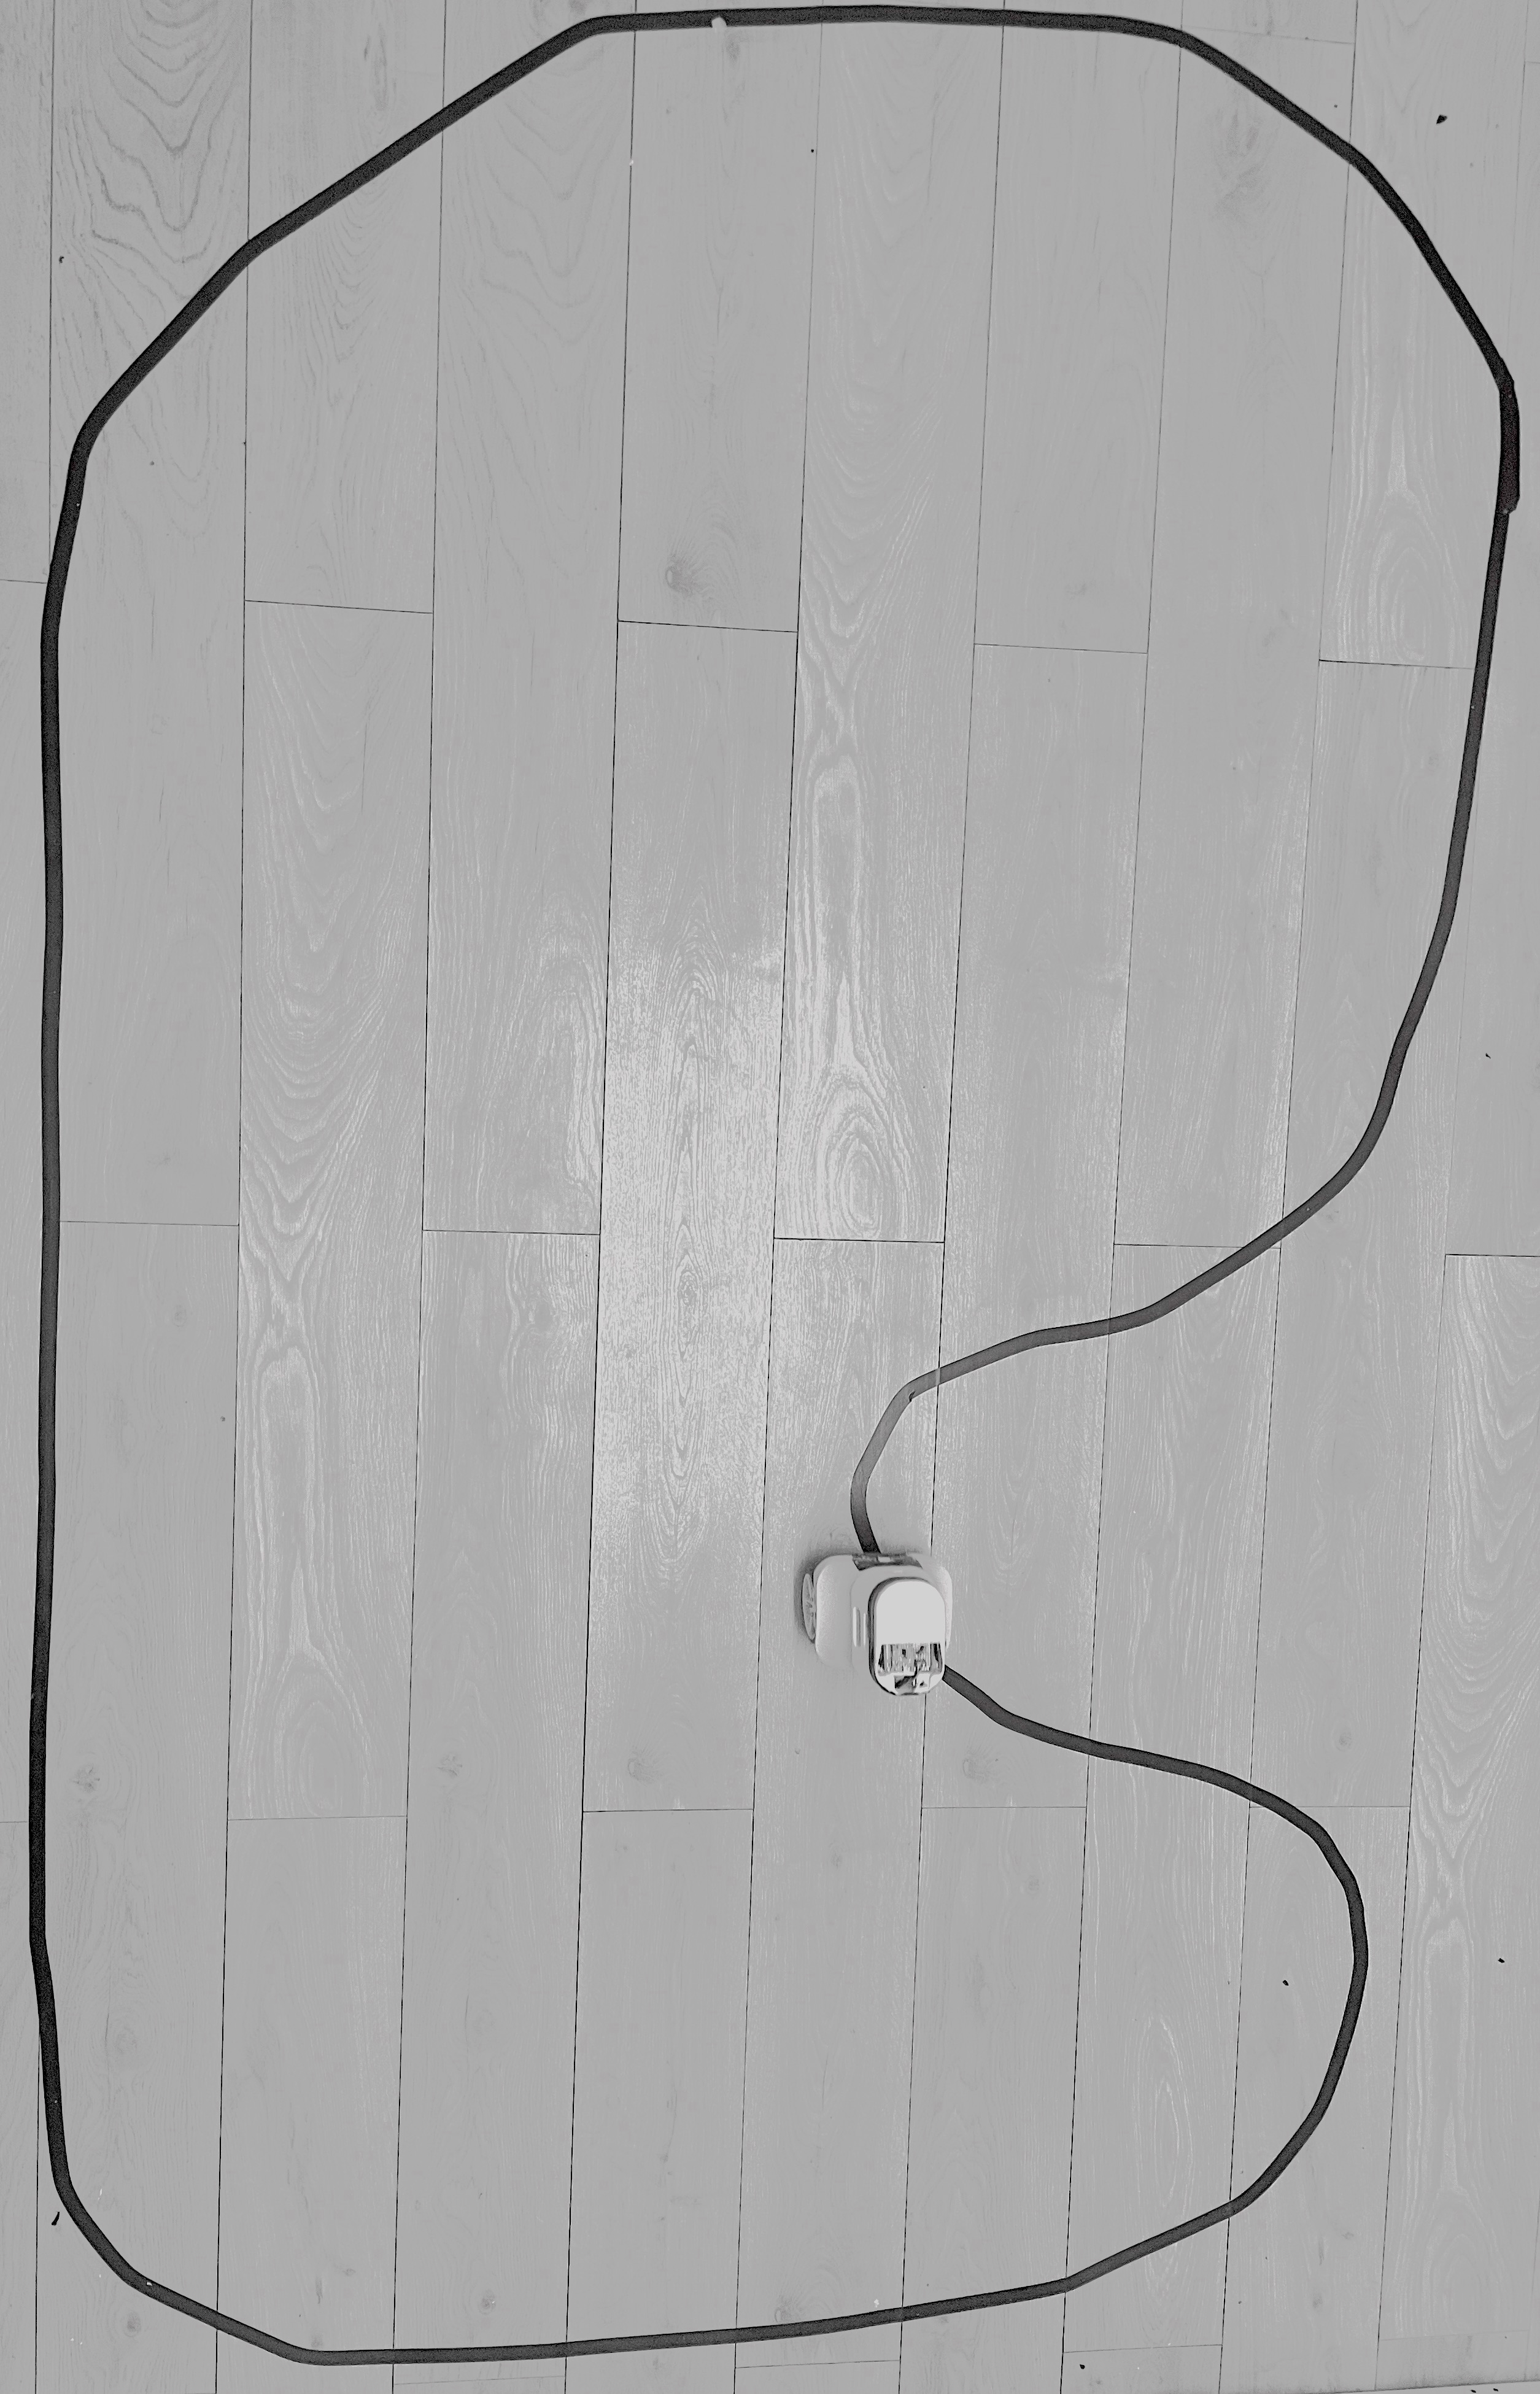
\includegraphics[height=\textwidth]{TrajTrak.jpeg}}  % Increase height for better visibility
            \caption{Race Track}
        \end{subfigure}
        \hspace{0.05cm}  % Adds horizontal space between the subfigures
        \begin{subfigure}[c]{0.6\textwidth}  % Adjusted width to match
            \centering
            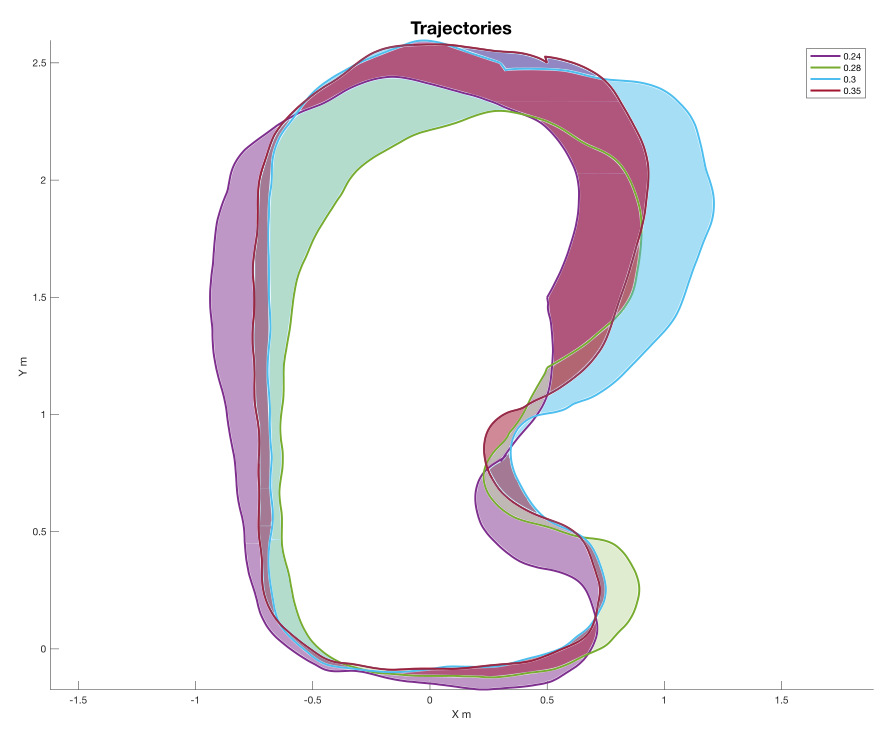
\includegraphics[width=\textwidth]{Graphs/DeadReckoningTrackMap.pdf}
            \caption{Map built offline using dead reckoning}
        \end{subfigure}
        \caption{Trajectory Tracking and Map Visualization}
    \end{figure}
    
    
    \pagebreak{}


  %%%%%%%%%%%%%%%%%% SECTION 4 %%%%%%%%%%%%%%%%%%
  \section{Results and discussion} % edit section heading as appropriate
    \subsection{Balance Performance}
    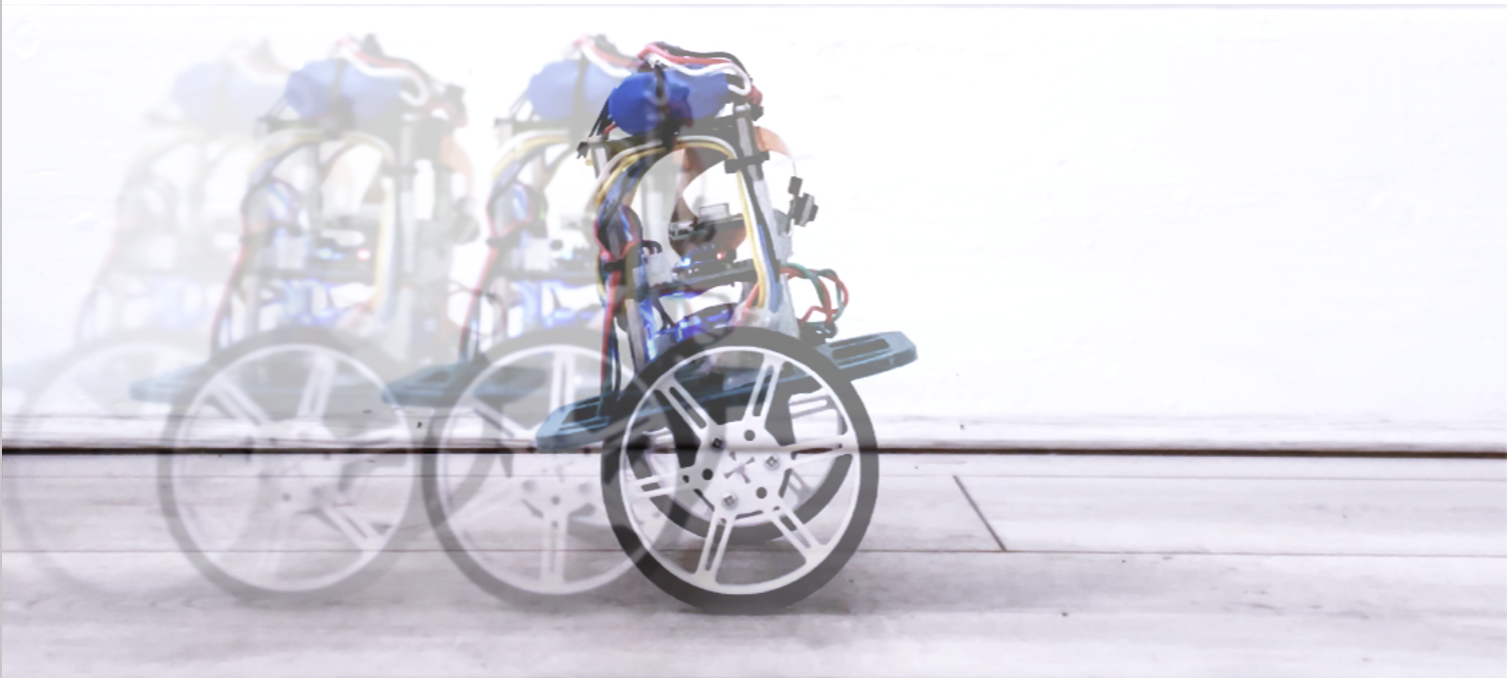
\includegraphics[width=\textwidth]{V1Colated.png}
    \subsection{Operational Robustness}
    \subsection{Line Trajectory Tracking}
    \subsection{More detail}
    \subsection{Summary}
  %%%%%%%%%%%%%%%%%% SECTION 5 %%%%%%%%%%%%%%%%%%
  \section{Conclusions and future work} % edit section heading as appropriate
    \subsection{Conclusions}
      \subsection{Future work}
  %%%%%%%%%%%%%%%%%% REFERENCES %%%%%%%%%%%%%%%%%%
    \printbibliography[title={References},heading=bibintoc] 
  %%%%%%%%%%%%%%%%%% APPENDICES %%%%%%%%%%%%%%%%%%
  \begin{uomappendix} 
      \section{Code}
      \section{Risk assessment}
      Risk assessment is a required appendix. Put here.
      %\section{Other appendices as necessary}
  \end{uomappendix}
  
  %%%%%%%%%%%%%%%%%% END MATTER %%%%%%%%%%%%%%%%%%
  \end{document}